\section{Конструкторская часть}
\subsection{Выбор языка программирования}
\subsubsection{Рассмотрение альтернатив}
Ниже приведены возможные варианты выбора языка, разделённые по классам, и оценка их применимости в задаче.
\begin{itemize}
    \item Относительно низкоуровневые компилируемые языки (\textit{C}, \textit{C++}). Применимость этих языков в основном ограничена сложностью и низкой скоростью разработки на них в связи с недостаточно высоким уровнем абстрактности этих языков. Высокая производительность, которой можно достичь с помощью них, не является серьёзным преимуществом, поскольку реализация работающей системы на таких языках занимает значительно большее время, делая разговор о конечной производительности преждевременным.
    \item Более высокоуровневые компилируемые языки (\textit{Java}, \textit{C\#}). Эти языки работают на виртуальных машинах, что ограничивает их переносимость. В случае \textit{C\#}, полная современная реализация существует только для Windows, что является неприемлимым в связи с тем, что конечная система должна работать и на Unix-подобных операционных системах. Ещё одним недостатком можно назвать их компилируемость, поскольку это опять же снижает скорость разработки и значительно усложняет реализацию интерактивного окружения для проведения экспериментов.
    \item Современные императивные интерпретируемые языки (\textit{Ruby}, \textit{Python}). Эти языки позволяют вести разработку с высокой скоростью и хорошо приспособлены для Test-Driven Development («разработка через тестирование», \cite{tdd}). Они хорошо переносимы и позволяют легко реализовать интерактивное окружение. Недостатком является относительно низкая скорость выполнения, что компенсируется более высокой скоростью разработки.
\end{itemize}
Другие семейства языков не рассматриваются ввиду низкой популярности. Это обусловлено тем, что язык реализации системы должен быть знаком большому количеству специалистов --- так будет проще вести  разработку.


\subsubsection{Итоговое решение}
В качестве основного языка реализации системы был выбран Python \cite{python}. Это простой и удобный, популярный и хорошо поддерживаемый язык с большим количеством библиотек. Он более распространён \cite{langpop} и имеет большее количество библиотек, чем Ruby. Он хорошо поддерживает современные методики разработки программ, такие, как TDD \cite{tdd}, за счёт встроенных модулей для работы с автоматическими тестами.

В случае необходимости можно достигнуть высокой производительности с помощью интерпретатора PyPy \cite{pypy}. Для реализации сложной обработки данных можно использовать модуль scipy \cite{scipy} и для визуализации \mbox{графиков --- модуль} matplotlib \cite{matplotlib}.


\subsection{Репозиторий исходных кодов экспериментальных программ}
Инструментарий выполняет эксперименты по оптимизации над программами, исходный код которых доступен экспериментатору. Экспериментатору должна быть доступна большая база исходных кодов для обеспечения возможности производить эксперименты над разнообразными программами, среди которых должны быть и похожие между собой. Последнее требование нужно ввиду необходимости обнаруживать похожесть программ в их оптимизационном поведении.

В качестве репозитория предлагается использовать сервер распределённой системы контроля версий \cite{distributed-vcs}. Такая архитектура позволяет удобно работать с локальными копиями репозитория при необходимости произвести незначительные изменения для проверки какой-либо гипотезы относительно оптимизационного поведения программ. Она также позволяет отправлять локальные изменения на центральный сервер, что полезно для обмена исходными кодами между экспериментаторами. В отличие от централизованной системы контроля версий, распределённая система позволяет удалённым участникам разработки легко включиться в процесс развития системы (во многом за счёт более простого и мощного процесса ветвления версий кода). Кроме того, она позволяет использовать для размещения репозитория бесплатные службы вроде {Github} \cite{github} и {Bitbucket} \cite{bitbucket}, что устраняет необходимость в выделенном сервере системы контроля версий.

\subsubsection{Рассмотрение альтернатив}
Далее рассматриваются основные распределённые системы контроля версий с оценкой их применимости в задаче. Основным источником является веб-страница \cite{git-vs-hg}.
\begin{itemize}
    \item {Mercurial}. Эта система контроля версий более проста в изучении и лучше поддерживает Windows. Вместе с тем, она в большей степени ограничивает разработчика --- например, не позволяет переписывать историю изменений.
    \item {Git}. Эта система версионирования является более мощной, чем {Mercurial} и позволяет производить многие необходимые в процессе работы действия более быстро и удобно.
\end{itemize}

\subsubsection{Итоговое решение}
В связи с большой гибкостью, в качестве репозитория исходных кодов был выбран {Git}. Это перевешивает недостаточную поддержку Windows, поскольку на данном этапе работы Windows не является приоритетной платформой для работы системы.

Стоит отметить, что на данный момент репозиторий исходных кодов тестовых программ является частью общего репозитория исходного кода описываемой системы. Этим также частично обусловлен выбор в пользу {Git}, поскольку исторически исходный код инструментария находился в {Git}.


\subsection{База данных экспериментов}
Для хранения данных об экспериментах необходима база данных. Традиционная реляционная база данных плохо подходит на эту роль, поскольку они требуют наличия жёсткой схемы, которой следуют все таблицы и все записи должны иметь одинаковый формат. Это представляет проблему в случае плохо определённой предметной области (такой, как наша исследовательская задача коллективной оптимизации), поскольку заранее неизвестно, какие свойства сущностей, сохраняемых в БД, являются важными, а какие --- нет. Это приводит к тому, что структура БД часто меняется по мере необходимости введения новых свойств, например, при добавлении нового признака исходного кода программы, по которому определяется похожесть одной программы на другую.

Рассмотрим документо-ориентированные базы данных. Они позволяют хранить документы в каком-либо текстовом формате (обычно JSON \cite{json}) и не требуют одинаковой структуры всех документов. Поля документов могут добавляться и удаляться непосредственно по запросу пользователя. Это свойство особенно важно для нашей задачи. Также эти БД лучше масштабируются (т.е. лучше приспособлены к использованию в крупных распределённых системах).

\subsubsection{Рассмотрение альтернатив}
Далее приведен список документо-ориентированных БД с оценкой их применимости в нашей задаче. Основой для сравнения служит источник \cite{nosql-comparison}.

\begin{itemize}
    \item MongoDB. Это хранилище во многом похоже на реляционные БД. Оно использует свой бинарный протокол передачи данных и ориентировано на получение высокой производительности.
    \item CouchDB. Это хранилище акцентировано на целостности хранимых данных и простоте в использовании. Оно поддерживает двустороннюю репликацию данных и представления данных через применение и свёртку (англ. "map-reduce"; см. источник \cite{map-reduce}). Также имеется возможность построения приложения на JavaScript, которое обеспечивает весь необходимый функционал БД (например, просмотр документов с определёнными свойствами). Хорошо подходит для ситуаций, когда данные накапливаются, но не изменяются.
    \item Redis. Хранилище в памяти для быстро-изменяющихся данных на протоколе, похожем на Telnet.
\end{itemize}

Другие альтернативы (HBase, Cassandra) не рассматриваются ввиду их специфичного фокуса на экстремально больших объёмах данных (типичных для банков и поисковых машин) и не лучшей поддержки интерфейса к языку {Python}.

\subsubsection{Итоговое решение}
В итоге в качестве БД была выбрана CouchDB, поскольку она хорошо подходит для сильно распределённых систем (что будет важно на дальнейших этапах работы) и накопления редко меняющихся данных. Поскольку в нашем случае эксперимент по оптимизации программы по определению не может быть изменён после проведения, это подходящий выбор.
Это хранилище также удобно в разработке --- оно позволяет удобно организовать все функции для доступа к данным в виде отдельного приложения на диске --- так называемого CouchApp \cite{couchapp}. Это позволяет хранить исходный код для работы с БД вместе с остальным исходным кодом инструментария.


\subsection{Установка инструментария на компьютер пользователя}
На данный момент установка происходит в ручном режиме. Необходимо скопировать (или получить из репозитория) исходный код инструментария на {Python}. Также необходимо установить интерпретатор {Python} версии не ниже 2.6, CouchDB версии не ниже 1.1 и CouchApp. В случае использования ОС Ubuntu или другой ОС Linux эта задача тривиально решается с помощью установки нужных бинарных пакетов с помощью пакетного менеджера, после чего никакой дополнительной настройки на данный момент не требуется.


\subsection{Расширяемость инструментария}
Инструментарий должен обеспечивать расширяемость в смысле возможности добавления новых модулей сборки, запуска и анализа данных. Это должно обеспечиваться описанием взаимодействия различных модулей системы. На данный момент эта задача не решается, поскольку более важным является получение результатов хотя бы на ограниченном множестве программ с фиксированным набором модулей сборки, запуска и анализа. На данный момент введение обобщённой архитектуры является преждевременным.

Однако стоит отметить базовую поддержку сценариев исследований. Сценарий --- это набор действий вида «собрать программу», «запустить программу с измерением времени», «построить график зависимости времени от компилятора» и т.д. Он может задаваться интерактивно или в исходном файле в виде функции языка программирования {Python} с использованием API инструментария в том же модуле, что и основной код системы, или в отдельном модуле (предпочтительно последнее). В будущем система будет также предоставлять интерфейс для использования её в качестве модуля языка {Python} сторонними пользователями. Полный набор доступных для использования в сценариях действий на данный момент описан только в исходном коде.

\subsection{Платформа для использования инструментария}
В идеальном варианте инструментарий должен поддерживать максимальное число различных программно-аппаратных платформ, как настольных, так и мобильных.

На начальном этапе инструментарий поддерживает ОС Linux на x86-совместимом процессоре ввиду распространённости данной аппаратной платформы, а также удобства разработки и ведения исследований под Linux.

\subsection{Архитектура инструметария}
Инструментарий состоит из нескольких основных компонентов. Они перечислены ниже.

\begin{itemize}
    \item Компонент загрузки и установки основных переменных. Этот компонент осуществляет инициализацию инструментария и выполняет получение базового пути к каталогу системы, соединяется с базой данных и передаёт управление определённому сценарию исследования или пользователю.
    \item Компонент поддержания структуры рабочих путей. Этот компонент работает со стеком путей и позволяет пользователю переходить к под-каталогам инструментария различными способами:
    \begin{itemize}
        \item от корня инструментария;
        \item от корня репозитория исходных кодов исследуемых программ;
        \item по абсолютному пути в локальной операционной системе.
    \end{itemize}
    \item Компонент подготовки команд для сборки и запуска программ. Он осуществляет шаблонную подстановку заданных пользователем значений в заготовки команд.
    \item Компонент запуска подготовленных команд и обмена данными с запущенным процессом. Он осуществляет запуск в контролируемом окружении, измерение времени работы и приём-передачу потоков стандартного ввода, вывода и ошибок.
    \item Компонент калибровки измерения времени. Его описание можно найти ниже в подразделе с соответствующим названием.
    \item Компонент сравнения измеренного времени с заведомо известным. Осущестляет вычисление ошибки измерения.
    \item Компонент создания документов базы данных из полученных в рамках эксперимента сведений. Документы имеют формат JSON \cite{json} и создаются из внутренних структур данных инструментария для возможности последующего сохранения в базу данных.
\end{itemize}

Все компоненты реализованы в виде функций языка {Python}. Применение объектной модели на данный момент не необходимо и перегружает код ненужными абстракциями.

\subsection{Эксперимент по оптимизации программы}
Эксперимент состоит в следующем.

\begin{enumerate}
	\item Система собирает программу с определёнными настройками сборки (см. ниже).

	\item Система запускает программу в контролируемом окружении с определёнными настройками запуска и производит измерение интересующих метрик исполнения программы. Список метрик см. ниже.

	На данный момент нас будет интересовать полное время исполнения.
	Список настроек исполнения см. ниже.

	\item Система сохраняет данные о сборке и запуске программы в базу данных для последующего анализа и обработки.
\end{enumerate}

В случае компилятора gcc настройки сборки включают в себя \cite{gcc-options}:
\begin{itemize}
    \item компилятор (команда для запуска);
    \item базовый уровень оптимизации (флаг '-O[n]', где n --- уровень оптимизации);
    \item набор флагов тонких настроек оптимизации (флаги семейства '-f[name]', где name --- имя определённого набора оптимизаций). Некоторые из этих флагов также имеют числовые параметры;
    \item путь к заголовочным файлам (опция '-I');
    \item путь к исходным файлам;
    \item параметры определения макросов (флаги вида '-D[MACRO]', где MACRO --- имя определяемого макроса);
    \item путь к исполняемому файлу, производимому компилятором.
\end{itemize}

Метрики исполнения могут включать в себя:
\begin{itemize}
    \item полное время исполнения программы;
    \item время исполнения программы по функциям;
    \item полный объём памяти, занимаемой программой и данными;
    \item объём памяти, занимаемой кодом программы;
\end{itemize}

\begin{samepage}
Настройки исполнения включают в себя:
\nopagebreak
\begin{itemize}
    \item путь к исполняемому файлу;
    \item источник ввода для стандартного потока ввода программы (перенаправление stdin);
    \item потоки вывода для стандартного потока вывода и стандартного потока ошибок программы (перенаправление stdout и stderr соответственно);
    \item аргументы запуска, в т.ч. путь к обрабатываемому файлу данных (например, путь к файлу изображения для программы сжатия изображений).
\end{itemize}
\end{samepage}


\subsubsection{Время исполнения программы}
Точное измерение времени исполнения программы может представлять сложности ввиду возможных колебаний из-за изменения загрузки системы другими задачами. Принципиально, рекомендуется выполнять эксперименты на системе, не занятой другими задачами. Однако даже в таком случае системные процессы или разница в решениях, принятых планировщиком процессов, могут оказать значительное воздействие на измерение времени. Подробнее о механизмах, применяемых в планировщиках процессов в современных ОС и о возможном воздействии на время выполнения задачи, смотри источник \cite{scheduling}.

Для устранения описанных проблем необходимо производить несколько запусков программы. Программа запускается 3 раза и берётся минимальное время её выполнения. Это время будет наиболее точно отражать производительность программно-аппаратной платформы, поскольку увеличение времени выполнения происходит в связи с интерференцией данного процесса с другими и общим состоянием системы. Как показали эксперименты (результаты в этой работе не приводятся), воздействие кэширования на производительность программы из тестового набора при многократном запуске при текущей реализации инструментария не наблюдается.

В случае внешнего измерения времени исполнения влияние оказывают также накладные расходы, связанные с запуском программы из системы. Для их исключения измерять время исполнения лучше изнутри программы и выводить его, например, в стандартный поток ошибок. Таким образом измерение времени производится в пакете тестирования производительности POLYBENCH \cite{polybench}.

Внутреннее измерение времени исполнения обеспечивает большую точность, однако, оно требует поддержки на уровне исходного кода. Очевидно, что для универсального инструментария запуска оптимизационных экспериментов такое решение неприемлемо, поскольку должно быть возможно измерение времени выполнения программ, никак специально не подготовленных для этого.

По этой причине система измеряет время исполнения извне. Невысокая точность измерения при этом устраняется с помощью калибровки (см. ниже). При этом также стоит отметить, что погрешность, вносимая внешним измерением, является систематической и не оказывает влияния на относительное время выполнения разных версий программы, что является наиболее важным в данной задаче.

\subsubsection{Калибровка времени исполнения программы}
\label{sssect:calibration}
Помимо отмеченных сложностей, есть сложность измерения маленьких интервалов времени. Если время исполнения программы находится на уровне 1 мс (таково временное разрешение системного вызова Unix $gettimeofday$), то даже если запускать программу несколько раз, колебания измерений окажутся настолько большими, что сделают результат неточным. Для устранения этой проблемы предлагается специальный алгоритм калибровки, схема которого приведена ниже. Он также позволяет уменьшить влияние колебаний времени исполнения.

\begin{enumerate}
    \item Положить $n = 0, t = 0, d_{rel} = 1$
    \item Исполнить программу однократно и измерить время её выполнения
    \item Если время выполнения более 1 секунды, положить $n = -1$
    \item Производить следующий цикл, пока $t < 1$ и $d_{rel} > 0,05$. Иначе перейти к шагу 9.
    \item Увеличить n на 1: $n = n + 1$
    \item Вычислить число запусков программы как $number = 10^{n}$
    \item Запустить программу $number$ раз, измеряя время выполнения. Повторить это 3 раза. Среди результатов выбрать минимум и присвоить его $t$. Вычислить относительную дисперсию результатов и присвоить её $d_{rel}$.
    \item Перейти к шагу 4.
    \item Получить время исполнения программы как $t / number$.
\end{enumerate}

В ряде случаев также используется сравнение измеренного времени исполнения с «реальным». Хотя на практике сложно измерить время реального исполнения (т.е. за исключением времени запуска), время запуска можно вычислить, запустив программу, которая ничего не делает, и измерив время её исполнения. Затем можно вносить поправку на время запуска в каждое измерение (для устранения систематической методической погрешности). Проблема этого решения в том, что требуется очень точное измерение времени запуска пустой программы, но при применении тех же методов это принципиально невозможно --- время её исполнения также будет сильно колебаться в зависимости от загрузки системы и практически случайного воздействия планировщика задач в текущем состоянии системы.

Оценку предложенных методов измерения времени можно произвести путём сравнения измеренного времени исполнения с временем, заданным таймером с помощью вызова функции $usleep$ стандартной библиотеки языка {С} изнутри программы.

Стоит отметить, что существуют постоянные расходы на запуск программы из нашей системы и их можно вычесть из измеренного времени для повышения точности измерения. Для этого мы вычисляем время выполнения пустой программы, а затем вычитаем его из каждого измеренного результата выполнения реальных программ.

\subsubsection{Интерактивное окружение проведения экспериментов}
Для удобной работы с инструментарием рекомендуется использовать интерпретатор ipython \cite{ipython}. Он предоставляет графическую оболочку языка {Python}, которая позволяет строить графики в том же окне, сохранять сессии использования интерпретатора и имеет хорошую поддержку автодополнения команд и документации. Ниже приведён снимок экрана этой графической оболочки с встроенным графиком.

\begin{figure}[H]
    \center{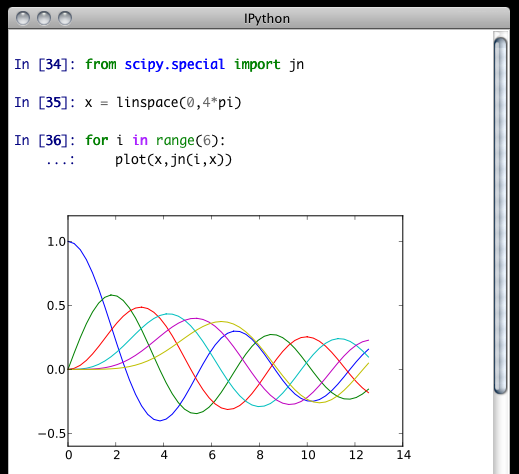
\includegraphics[width=0.6\linewidth]{besselj}}
    \caption{Cнимок экрана графической оболочки IPython с встроенным графиком.}
\end{figure}
